\chapter{Materiais e Métodos\label{cap:metodologia}}

	A metodologia teve três pilares: sólida base em Algoritmos Genéticos, estudo detalhado dos artigos e desenvolvimento de um \emph{software} confiável para execução do modelo. Os três são apresentados nas seções seguintes.

%========================================================
\section{Algoritmos Genéticos}\label{seq:medologia_ga}
%========================================================
	
	Iniciei os estudos em Algoritmos Genéticos pelos livros \cite{Mitchell98} e \cite{Linden2008} e, antes de partir para o trabalho da dissertação em si, ataquei três problemas completamente distintos.
	
	O primeiro foi o ONEMAX \cite{onemaxNaGPU}, desenvolvido ``do zero'', em Linguagem C. Considerado o \emph{hello world} do GA, tem representação cromossomial binária, o \emph{fitness} é a soma dos \emph{bits} de cada indivíduo e o objetivo é obter um indivíduo com o maior número de '1' possível. Com ele pude estudar os parâmetros de um GA simples, como número de indivíduos e a probabilidade de \emph{crossover}, e verificar a influência de cada um na qualidade da solução, convergência, desempenho, evolução do \emph{fitness} etc. Uma versão paralelizada em CUDA foi apresentada em evento de computação de alto desempenho \cite{ERAD12} e é discutida na seção \ref{sec:oneMaxNaGPU}.
	
	\begin{figure}[htbp]
		\centering
			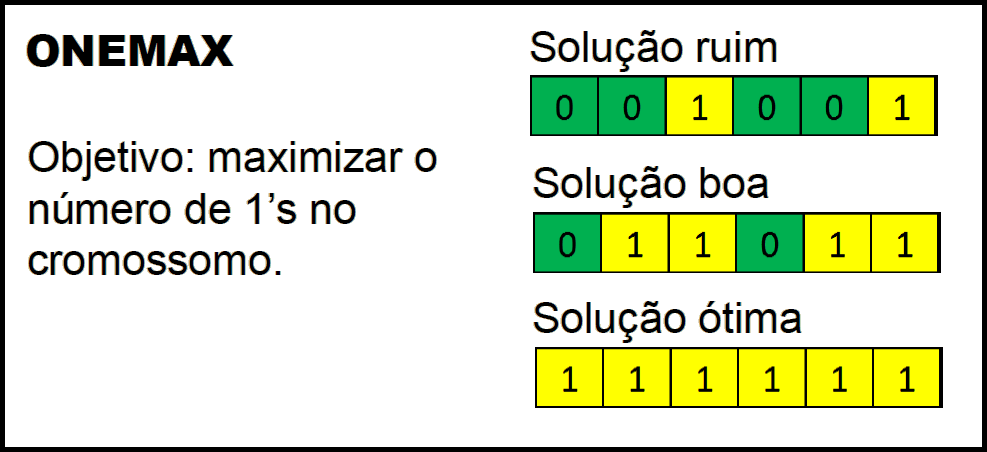
\includegraphics[width=0.60\textwidth]{figs/resultados/onemax/onemax_objetivo.png}
		\caption{ONEMAX: representação cromossomial, \emph{fitness} e objetivo.}
		\label{fig:onemax_objetivo_metodologia}
	\end{figure}
	
	Tendo a estrutura básica do ONEMAX, o próximo passo foi tentar fazer um modelo. Abordei o Problema das Oito Rainhas, que consiste em posicionar oito rainhas em um tabuleiro de xadrez de modo que não se ataquem. Sem nenhuma referência externa, propus um modelo de GA que conseguiu chegar em algumas soluções \cite{qualificacao_adriano}. Uma delas está na figura \ref{fig:OitoRainhasSolucao}.
	
	\begin{figure}[htbp]
		\centering
			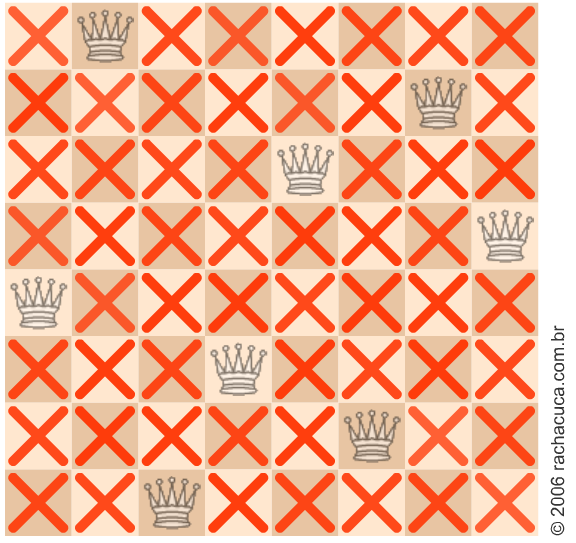
\includegraphics[width=0.30\textwidth]{figs/materiais_metodo/ga/OitoRainhasSolucao.png}
		\caption{Uma solução para o Problema das 8 Rainhas.}
		\label{fig:OitoRainhasSolucao}
	\end{figure}
	
	Tratando o tabuleiro de xadrez como um plano cartesiano, a representação cromossomial era um \emph{string} com os oito pares de coordenadas $(x,y)$. Cada coordenada gerava uma matriz característica de 0's e 1's que, quando somadas, resultava em uma matriz com a informação da quantidade $c$ de ataques que cada rainha sofreu. O objetivo, portanto, era encontrar um indivíduo que levasse a $c = 0$. A função de avaliação foi definida como $f = 1/(1 + c)$.
	
	Criar um modelo para o Oito Rainhas foi importante para o entendimento do elo entre um GA e o problema a ser resolvido. Essa ligação encontra-se na representação cromossomial e na função de avaliação. Defini ambas de maneira adequada, mas a representação cromossomial apresentou um problema: nada impede de haver pontos $(x,y)$ repetidos no cromossomo. Em outras palavras, ela permite que duas rainhas sejam colocadas na mesma posição do tabulareiro, o que é proibido no xadrez. 
	
	Por fim, utilizei GA na criação de um robô, chamado \emph{Genético}, para ser testado contra os campeões do torneio de Robocode da Faculdade de Tecnologia da Unicamp\footnote{\texttt{http://torneiorobocode.orgfree.com/torneio-ft.php}}. Robocode é um jogo\footnote{\texttt{http://robocode.sourceforge.net/}}, cujo objetivo é programar um tanque de guerra robô para competir contra outros robôs em uma arena de batalha. Ele começou como um projeto pessoal no ano 2000 e depois foi incorporado pela IBM\footnote{\texttt{http://robocode.sourceforge.net/docs/ReadMe.html}}. Atualmente é um projeto de código aberto.
	
	\begin{figure}[htbp]
		\centering
			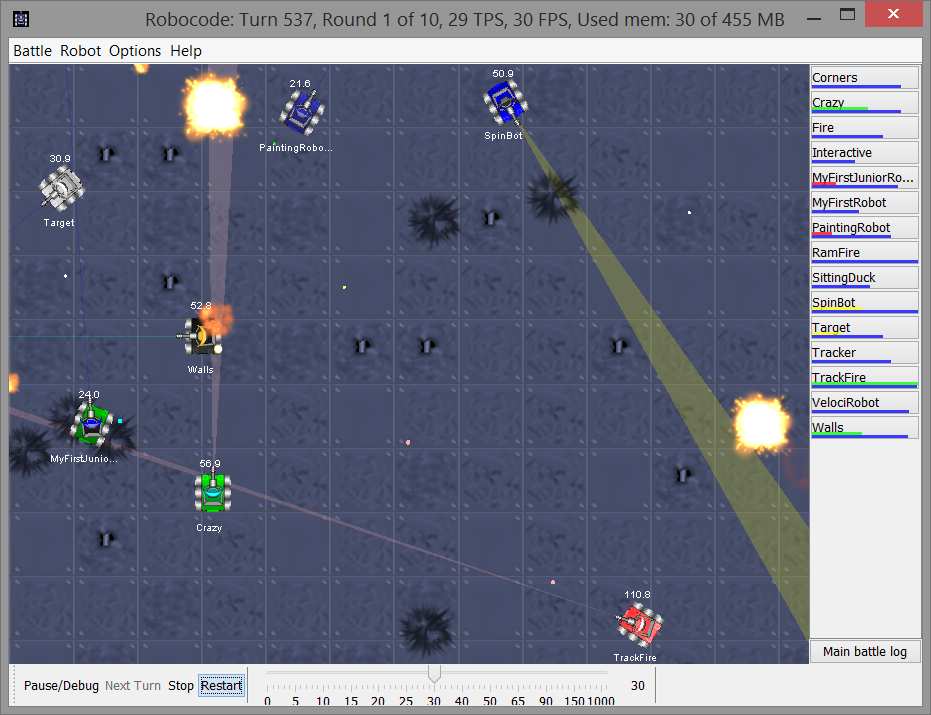
\includegraphics[width=0.50\textwidth]{figs/materiais_metodo/ga/Robocode_Battle_Field.PNG}
		\caption{Arena de batalha do Robocode.}
		\label{fig:Robocode}
	\end{figure}
	
	Me baseei no artigo \cite{robocodeGA}, publicado em um congresso de computação evolutiva da IEEE. As primeiras versões do \emph{Genético} não travaram boas batalhas. Alterei o \emph{fitness} e o processo de treinamento. Na versão final o ele foi capaz de vencer os robôs que ficaram em primeiro e terceiro lugar no torneio daquele ano (o segundo lugar não estava disponível para \emph{download}). O \emph{Genético} vencia, inclusive, contra os dois simultaneamente \cite{robocodeGA_adriano}.
	

%========================================================
\section{\emph{Software}}
%========================================================

	O \emph{software} utilizado foi totalmente desenvolvido por mim, e há razões metodológicas que justificam essa escolha. Obtive bons resultados criando os próprios programas nos estudos iniciais de GA. Eles foram fundamentais para que eu soubesse exatamente o que estava acontecendo durante a execução. Quis ter esse controle total também sobre o programa que executaria o GA proposto para essa dissertação. Ele foi escrito em Linguagem C, utilizando apenas quatro bibliotecas padrão: \texttt{stdio.h}, \texttt{stdlib.h}, \texttt{time.h} e \texttt{math.h}. Portanto, é totalmente portável para os sistemas operacionais que possuem um compilador C$++$. Além disso, C é a linguagem nativa da arquitetura CUDA, o que facilitará sua paralelização.
	
	Tive muito cuidado com a confiabilidade dos resultados. Quando opta-se por não gerá-la automaticamente, a \emph{semente} dos números pseudo-aleatórios é um dos parâmetros de entrada. Duas execuções com os mesmos parâmetros, incluindo a semente, levam a exatamente os mesmos resultados. Por isso nas tabelas e gráficos deixei explícito seu valor. Os gráficos encontrados em \cite{metodo2004} e \cite{metodo2011} referem-se ao maior \emph{fitness} (e $\rho$ associado) de cada geração. O programa gera essa informação, mas também exibe as médias dessas variáveis. De acordo com \cite{Mitchell98}, uma teoria geral para entender e prever o comportamento dos GAs seria análoga à Mecânica Estatística na Física. Ao contrário de lidar com grande número de componentes do sistema, como a composição genética exata de cada população, tal abordagem trabalha com uma estatística mais ``macroscópica'', como o \emph{fitness} médio da população. Portanto, tanto os critérios de parada do programa quanto a minha análise foram baseadas em médias.
	
	Para utilizar o \emph{software} basta baixar o código e compilar o arquivo \texttt{Serial\_novo.c} (será necessário alterar o diretório no \emph{include} das bibliotecas que desenvolvi). O código está disponível na internet para qualquer um utilizar, testar e, inclusive melhorar\footnote{\texttt{https://github.com/prietoab/msc\_code}}. Caso isso aconteça, peço apenas que cite essa dissertação.
	
		A execução se dá via linha de comando passando os parâmetros necessários. Porém, como são muitos parâmetros, é aconselhável a utilização de um arquivo de \emph{script}. Assim é possível criar processos de varredura para variar os parâmetros desejados ou repetir várias execuções. Fiz isso para automatizar o estudo e ter dados suficientes para análise. Na figura \ref{fig:script_windows} há um exemplo de \emph{script} Windows para fazer execuções variando o número de genes.
			
		\begin{figure}[htbp]
			\centering
				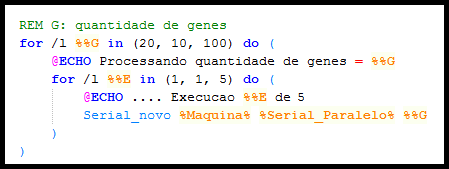
\includegraphics{figs/materiais_metodo/software/script_windows.png}
			\caption{Exemplo de \emph{script} Windows para fazer execuções variando o número de genes.}
			\label{fig:script_windows}
		\end{figure}

	Não é necessário ter uma matriz para execução. Através do parâmetro \emph{Tamanho do cromossomo} (seção \ref{sec:listaParametros}) o programa gera automaticamente uma matriz de Coope \cite{Coope1977}, definida na equação \ref{eq:MatrizCoope}. Essa matriz foi utilizada nos testes de \cite{metodo2011}.
	
	\begin{equation}\label{eq:MatrizCoope}
		\begin{array}{ccl}
			H(i,i) = 2i - 1 			& , & i = 1, 2, ..., n. \\
														&		&		\\
			H(i,j) = H(j,i) = 1		& , & i \neq j; \\
														&		& i = 1, 2, ..., n; \\
														&		& j = 1, 2, ..., n.
		\end{array}
	\end{equation}
	
%---------------------------------------------------
\subsection{Informações de saída}
%---------------------------------------------------	
		
Há cinco grupos de informações na saída do programa. Usados em conjunto dão um panorama geral do algoritmo genético. Para apenas um deles (Estatística) um arquivo texto é gerado automaticamente. Os outros são exibidos na tela. Para alterar a saída padrão para um arquivo texto, é necessário utilizar o caractere de redirecionamento da saída padrão. No Windows, Linux e Unix esse caractere é o ``>''. No Linux, por exemplo, o comando ``\texttt{ls > dirs.txt}'' lista o conteúdo do diretório atual e armazena no arquivo \texttt{dirs.txt}.

\begin{enumerate}

	\item \textbf{Cabeçalho}
	
		Contém todos os parâmetros de execução recebidos na linha de comando. Impresso na tela.
	
	\item \textbf{Comportamento do \emph{fitness}}
	
		Imprime na tela, para cada geração, além de alguns parâmetros de execução, as seguintes informações: 
		
		\begin{itemize}
			\item $\rho$ mínimo
			\item $\rho$ médio (<$\rho$>)
			\item \emph{fitness} médio (<\emph{fitness}>)
			\item Maior \emph{fitness}
			\item $\rho$ associado ao maior \emph{fitness}
			\item <$|\nabla \rho|^2$>
			\item Posição do melhor indivíduo
		\end{itemize}

	\item \textbf{Tempos de processamento}
	
		Imprime na tela uma estimativa para o tempo de processamento (em \emph{clocks}) para cada operador. Se o programa foi executado por 200 gerações, haverá 200 tempos de processamento para o \emph{fitness}, seleção, \emph{crossover} e mutação.
		
	\item \textbf{Geração final}
	
				Impressão de todos os indivíduos da última geração. 
	
	\item \textbf{Estatística}
	
				A cada execução é criado (ou atualizado caso já exista) um arquivo chamado \texttt{estatistica.txt}. Nele, além de todos os parâmetros, há informações relacionadas à geração que atingiu algum critério de parada. Por exemplo, além do próprio número da última geração, há o \emph{fitness} médio, o maior \emph{fitness}, o $\rho$ associado ao maior \emph{fitness}, o $\rho$ médio e o tempo total de processamento do programa.
	
\end{enumerate}
	
%---------------------------------------------------
\subsection{Lista dos arquivos fonte}
%---------------------------------------------------
	
	O programa é pequeno ($\approx$ 2500 linhas), e está distribuído em seis arquivos, um principal e cinco bibliotecas:
	
	\begin{itemize}
		\item \textbf{Serial\_novo.c}
		
		Arquivo principal. Contém o fluxo do GA (figura \ref{fig:fluxo}).
		
		\item \textbf{Estruturas.h}
		
		Contém as estruturas de dados e uma função que retorna automaticamente o parâmetro $\lambda$ do \emph{fitness} (seção \ref{sec:eq_lambda}).
		
		\item \textbf{Algebra\_Linear\_serial.h}
		
		Mutiplicação e subtração de matrizes.
		
		\item \textbf{Estatistica.h}
		
		Média, variância e desvios do Quociente de Rayleigh.
		
		\item \textbf{Auxiliares\_serial.h}
		
		Números pseudo-aleatórios, alocação de memória para indivíduos na população.
		
		\item \textbf{GA\_Serial.h}
		
		Contém as funções do Algoritmo Genético. A maoria do código está nessa biblioteca.	
		
	\end{itemize}
					
%---------------------------------------------------
\subsection{Lista dos parâmetros de execução}
\label{sec:listaParametros}
%---------------------------------------------------
	\begin{enumerate}
		\item \textbf{Código da máquina}.
		
				Número inteiro, utilizado para identificar o computador que o programa foi executado. Útil para comparar as execuções em computadores diferentes. Por exemplo, se há quatro computadores A, B, C e D, é possível classificá-los como A = 0, B = 1, C = 2, D = 3.
				
		\item \textbf{Serial ou Paralelo}?
		
				Número inteiro. Determina se a execução será serial (= 0) ou paralela (= 1). A atual versão permite apenas execução serial. Portanto, esse parâmetro pode ser fixado em zero.
				
		\item \textbf{Tamanho do cromossomo (ordem da matriz de Coope)}.
		
				Número inteiro. Determina a ordem da matriz de Coope. Inserir 200 nesse parâmetro gera uma matriz de Coope de tamanho 200 x 200.
			
		\item \textbf{Quantidade máxima de gerações}.
		
				Número inteiro. Um dos critérios de parada. Para evitar que o programa entre em um \emph{loop} infinito caso não haja convergência para uma solução. Se definida como 100, o programa executará, no máximo, 100 iterações de Avaliação, Seleção, \emph{Crossover} e Mutação.
		
		\item \textbf{Quantidade de indivíduos na população}.
		
		Número inteiro. Determina a quantidade de indivíduos em cada população.
		
		\item \textbf{Tipo do Fitness}.
		
		Número inteiro. O programa pode trabalhar com cinco tipos de \emph{fitness}. Dois deles são os apresentados na seção \ref{sec:fitness_metodo}. Qualquer código diferente dos apresentados abaixo faz com que o \emph{fitness} seja definido como $f = -1$.
		
			\begin{itemize}
				\item Tipo  0:
				
					\begin{equation}
					f = e^{-\lambda(\rho - E_L)^2}
					\end{equation}
				
				\item Tipo 1:
				
					\begin{equation}
					f = e^{-\lambda |\nabla \rho|^2}
					\end{equation}
					
				\item Tipo 2:
				
					\begin{equation}
					f = e^{-\lambda [(\rho - E_L)^2 + |\nabla \rho|^2]}
					\end{equation}
					
				\item Tipo 3:
				
					\begin{equation}
					f = e^{-\lambda |\nabla \rho|}
					\end{equation}
		
			\item Tipo 4:
				
					\begin{equation}
					f = e^{-\lambda [(\rho - E_L)^2 + |\nabla \rho|]}
					\end{equation}
			\end{itemize}
			
		\item \textbf{Tipo do Fitness Paralelo}.
		
				Número inteiro. A atual versão permite apenas execução serial. Portanto, esse parâmetro pode ser fixado em zero.
		
		\item \textbf{Tamanho do Torneio}
		
			Número inteiro. Define a quantidade de indivíduos selecionados para o torneio na Seleção.
		
		\item \textbf{Probabilidade do \emph{Crossover}}.
		
			Número real. Define, em porcentagem, a probabilidade de \emph{Crossover}. Exemplo: 80.5 = 80.5\%.
		
		\item \textbf{Quantidade de Pontos de Corte}.
		
			Número inteiro. Na versão atual a quantidade de pontos de corte foi fixada em dois conforme o operador de \emph{crossover} definido na seção \ref{sec:crossover_utilizado}. Pode ser mantido como zero.
		
		\item \textbf{Probabilidade de Mutação}.
		
		Número real. Define, em porcentagem, a probabilidade de mutação. Exemplo: 12.7 = 12.7\%.
		
		\item \textbf{Intensidade da Mutação - $\Delta$}.
		
			Número real. Define o parâmetro $\Delta$ utilizado no \emph{crossover}. É dividido por dez. Exemplo: $1.2$ no parâmetro $\rightarrow 0.12$ no $\Delta$.
		
		\item \textbf{Valor para $\lambda$}.
		
		Número real. Define o valor do parâmetro $\lambda$ do \emph{fitness}. Se for configurado como $-1$, um valor adequado para $\lambda$ é gerado automaticamente.
		
		\item \textbf{Valor para $E_L$}.
		
		Número real. Define um limite inferior para o autovalor mínimo ($E_0$) nos \emph{fitness} de tipo 0, 2 e 4. 
		
		\item \textbf{Precisão - $\xi$}.
		
		Número real. Define a precisão dos critérios de parada. O programa termina se a variável alvo é menor ou igual a $\xi$. Depende do tipo de \emph{fitness}.
		
		Condições de parada em função do \emph{fitness} ($<x>$ significa valor médio de $x$):
				
		\begin{itemize}
			\item Fitness tipos 0, 2 e 4:
			
			\begin{equation}
				\begin{array}{ccll}
				<|\nabla \rho_i|^2> & \leq & \xi & \mbox{  ou} \\
				| <\rho_i> - E_L | & \leq & \xi &
				\end{array}
			\end{equation}
			
			
			\item Fitness tipos 1 e 3:
			
			\begin{equation}
				\begin{array}{ccll}
					<|\nabla \rho_i|^2> & \leq & \xi &
				\end{array}
			\end{equation}
			
		\end{itemize}
		
		\item \textbf{Imprime comportamento do \emph{Fitness}}?
		
		Se configurado como Verdadeiro (1), imprime na saída padrão as variáveis de interesse para estudar o comportamento do \emph{fitness}. 
		
			0: \emph{Falso}. Não imprime.
			
			1: \emph{Verdadeiro}. Imprime.
		
		\item \textbf{Imprime tempos de execução}?
		
			Número inteiro. Se configurado como Verdadeiro (1), imprime na saída padrão os tempos estimados de execução (em \emph{clocks} do processador) das funções e operadores.
			
			
			0: \emph{Falso}. Não imprime.
			
			1: \emph{Verdadeiro}. Imprime.
			
		
		\item \textbf{Gera nova semente para números pseudo-aleatrórios}?
		
		Número inteiro. Se configurado como Verdadeiro (1), o programa cria uma nova semente para os números pseudo-aleatórios. Caso contrário, a semente definida no próximo parâmetro é utilizada.
		
		0: \emph{Falso}. Utiliza semente definida no parâmetro \emph{Semente}.
		
		1: \emph{Verdadeiro}. Cria uma nova semente. O parâmetro \emph{Semente} é ignorado.
		
		\item \textbf{Semente dos números pseudo-aleatrórios}.
		
		Número inteiro. Define a semente dos números pseudo-aleatórios. Depende do parâmetro anterior.
		
		\item \textbf{Tipo do cálculo de $\nabla \rho$}.
		
		Deve ser configurado como 1.
		
		Nas versões iniciais $\nabla \rho$ era calculado literalmente como na equação \ref{eq:grad_rho_metodo}, exigindo o uso de uma matriz identidade ($I$) da ordem do Hamiltoniano. A equação foi reescrita internamente de modo que $I$ não fosse necessária, liberando memória e fazendo menos operações. Usar ou não $I$ leva aos mesmos resultados.
		
		0: Utiliza matriz identidade.
		
		1: Não utiliza matriz identidade (libera memória e faz menos operações).
		
	\end{enumerate}